\documentclass[11pt]{beamer}
\usepackage[utf8]{inputenc}
\usepackage[T1]{fontenc}
\usepackage{lmodern}
\usepackage[english]{babel}
\usetheme{Darmstadt}
\setbeamertemplate{navigation symbols}{}
\setbeamertemplate{footline}{
	\begin{beamercolorbox}[ht=3ex,leftskip=1.4cm,rightskip=.3cm]{author in head/foot}
		\hfill \insertframenumber
		\vspace*{0.07cm}
	\end{beamercolorbox}
} 
\usepackage{url}
\usepackage{hyperref}

% color def
\usepackage{color}
\definecolor{darkred}{rgb}{0.6,0.0,0.0}
\definecolor{darkgreen}{rgb}{0,0.50,0}
\definecolor{lightblue}{rgb}{0.0,0.42,0.91}
\definecolor{orange}{rgb}{0.99,0.48,0.13}
\definecolor{grass}{rgb}{0.18,0.80,0.18}
\definecolor{pink}{rgb}{0.97,0.15,0.45}

\usepackage{listings}

\lstdefinestyle{Python}{
    language=Python,
    morekeywords=[1]{,as,assert,nonlocal,with,yield,self,True,False,None,} % Python builtin
	morekeywords=[2]{,__init__,__add__,__mul__,__div__,__sub__,__call__,__getitem__,__setitem__,__eq__,__ne__,__nonzero__,__rmul__,__radd__,__repr__,__str__,__get__,__truediv__,__pow__,__name__,__future__,__all__,}, % magic methods
	morekeywords=[3]{,object,type,isinstance,copy,deepcopy,zip,enumerate,reversed,list,set,len,dict,tuple,range,xrange,append,execfile,real,imag,reduce,str,repr,}, % common functions
	morekeywords=[4]{,Exception,NameError,IndexError,SyntaxError,TypeError,ValueError,OverflowError,ZeroDivisionError,}, % errors
	morekeywords=[5]{,ode,fsolve,sqrt,exp,sin,cos,arctan,arctan2,arccos,pi, array,norm,solve,dot,arange,isscalar,max,sum,flatten,shape,reshape,find,any,all,abs,plot,linspace,legend,quad,polyval,polyfit,hstack,concatenate,vstack,column_stack,empty,zeros,ones,rand,vander,grid,pcolor,eig,eigs,eigvals,svd,qr,tan,det,logspace,roll,min,mean,cumsum,cumprod,diff,vectorize,lstsq,cla,eye,xlabel,ylabel,squeeze,}, % numpy / math
	morestring=*[d]{"},
    basicstyle=\ttfamily,
   	backgroundcolor=\color{white},
   	commentstyle=\color{darkgreen}\slshape,
   	keywordstyle=\color{blue}\bfseries\itshape,
   	keywordstyle=[2]\color{blue}\bfseries,
   	keywordstyle=[3]\color{grass},
   	keywordstyle=[4]\color{red},
   	keywordstyle=[5]\color{orange},
   	stringstyle=\color{darkred},
   	emphstyle=\color{pink}\underbar,
    % honek neretako bakarrik die
    deletekeywords=[2]{next,set},
    deletekeywords=[3]{next,set},
}

% General Setting of listings
\lstset{
    style=Python,
	tabsize=4,
	aboveskip=1em,
	breaklines=true,
	abovecaptionskip=-6pt,
	captionpos=b,
	escapeinside={\%*}{*)},
	frame=single,
	numbers=left,
	numbersep=8pt,
	numberstyle=\tiny,
}

\usepackage{tikz}
\usetikzlibrary{calc,shapes.multipart,chains,arrows,positioning}

\tikzset{
	squarecross/.style={
		draw, rectangle,minimum size=18pt, fill=orange!80,
		inner sep=0pt, text=black,
		path picture = {
			\draw[black]
			(path picture bounding box.north west) --
			(path picture bounding box.south east)
			(path picture bounding box.south west) --
			(path picture bounding box.north east);
		}
	},
	list/.style={
		very thick, rectangle split,
		rectangle split parts=2, draw,
		rectangle split horizontal, minimum size=18pt,
		inner sep=4pt, text=black,
		rectangle split part fill={red!20, blue!20}
	},
	->, start chain, very thick,
	chain_arrow/.style={*->, thick}
}


\begin{document}
	\author{Data Structures}
	\title{Linked Lists}
	\titlegraphic{
\includegraphics[width=3cm]{img/UPNA}}
	\date[]{2024-2025}
	\subject{Data Structures}
	%\subtitle{}
	%\logo{}
	%\institute{}
	%\date{}
	%\subject{}
	%\setbeamercovered{transparent}
	%\setbeamertemplate{navigation symbols}{}
	\begin{frame}[plain]
		\maketitle
	\end{frame}

	\begin{frame}
		\tableofcontents
	\end{frame}

\section{What is a Linked List}

	\begin{frame}
		\frametitle{Overview of a Linked List}
		\begin{itemize}
			\item A list is a collection of elements
			\item In a \textbf{Linked List} each element in the list will point to the next element
			\item Each element is called a \textbf{Node}
			\item A Node will contain two variables
			\begin{itemize}
				\item The data we want to store
				\item The \textit{reference} to the next Node
			\end{itemize}
		\end{itemize}
		\vspace{1cm}
		\begin{center}
			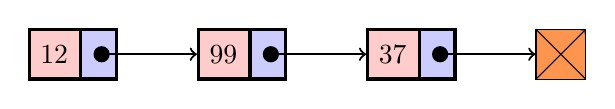
\begin{tikzpicture}
				\node[list,on chain] (A) {12};
				\node[list,on chain] (B) {99};
				\node[list,on chain] (C) {37};
				\node[squarecross]   (D) [right=of C] {};
				\draw[chain_arrow] let \p1 = (A.two), \p2 = (A.center) in (\x1,\y2) -- (B);
				\draw[chain_arrow] let \p1 = (B.two), \p2 = (B.center) in (\x1,\y2) -- (C);
				\draw[chain_arrow] let \p1 = (C.two), \p2 = (C.center) in (\x1,\y2) -- (D);
			\end{tikzpicture}
		\end{center}
	\end{frame}

	\begin{frame}[fragile]
		\frametitle{How to Create a Node}
		\begin{itemize}
			\item A Node will contain two points of data
			\begin{itemize}
				\item The data we want to store
				\item The reference to the next element
			\end{itemize}
			\item We can use a simple list to store it \lstinline|[data, next]|
			\item But it is easier to use a class
		\end{itemize}
\pause
\begin{lstlisting}
class Node:
	def __init__(self, data, next = None):
		self.data = data
		self.next = next
\end{lstlisting}
	\end{frame}

	\begin{frame}[fragile]
		\frametitle{Adding Relations to Nodes}
		\begin{itemize}
			\item Once we have created a Node to store our data we can start chaining them together
			\begin{itemize}
				\item The same way links in a chain work
			\end{itemize}
			\item We can create nodes and join them together with the next attribute
		\end{itemize}
		\vspace{0.5cm}
  		\begin{center}
  			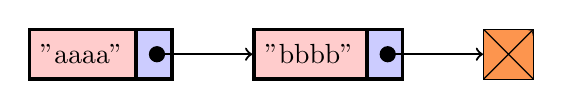
\begin{tikzpicture}
  				\node[list,on chain] (A) {\lstinline|"aaaa"|};
  				\node[list,on chain] (B) {\lstinline|"bbbb"|};
  				\node[squarecross]   (D) [right=of B] {};
  				\draw[chain_arrow] let \p1 = (A.two), \p2 = (A.center) in (\x1,\y2) -- (B);
  				\draw[chain_arrow] let \p1 = (B.two), \p2 = (B.center) in (\x1,\y2) -- (D);
  			\end{tikzpicture}
  		\end{center}
        \vspace{0.2cm}
        \pause
\begin{lstlisting}
first = Node("aaaa")
second = Node("bbbb")

first.next = second
\end{lstlisting}
		
	\end{frame}

	\begin{frame}
		\frametitle{Constructing the Linked List}
		\begin{itemize}
			\item We have created Nodes and linked them by defining the next node
			\item But having to change the value of the next attribute of the last element in the list is cumbersome
			\item The following step is to provide a interface similar to lists in Python
			\begin{itemize}
				\item Insert an element (at the head, tail or middle)
				\item Remove an element
				\item Get an element
				\item Get list size
				\item Check if an element exists in the list
				\item ...
			\end{itemize}
		\end{itemize}
		\vspace{0.7cm}
		\begin{center}
			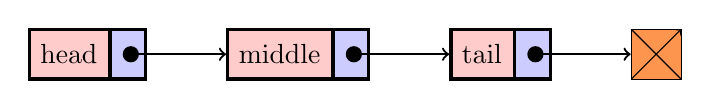
\begin{tikzpicture}
				\node[list,on chain] (A) {head};
				\node[list,on chain] (B) {middle};
				\node[list,on chain] (C) {tail};
				\node[squarecross]   (D) [right=of C] {};
				\draw[chain_arrow] let \p1 = (A.two), \p2 = (A.center) in (\x1,\y2) -- (B);
				\draw[chain_arrow] let \p1 = (B.two), \p2 = (B.center) in (\x1,\y2) -- (C);
				\draw[chain_arrow] let \p1 = (C.two), \p2 = (C.center) in (\x1,\y2) -- (D);
			\end{tikzpicture}
		\end{center}
	\end{frame}

	\begin{frame}[fragile]
		\frametitle{Using a Class for the Linked List}
		\begin{itemize}
		\item We can create a class that will handle the operations for us
		\item The class will have an attribute that references the head of the list
			\begin{itemize}
				\item The following elements can be reached jumping from a node to another
				\item Always starts at the head
			\end{itemize}
		\item We will work with the linked list, and not with individual nodes
		\end{itemize}
\begin{lstlisting}
class Linked_list:
	def __init__(self, head = None):
		self.__head = head
\end{lstlisting}
	\end{frame}

\section{Basic Functions}

	\begin{frame}[fragile]
		\frametitle{Getting the Size}
		\begin{itemize}
			\item \lstinline|linked_list.size()|
			\item Starting from the head \textbf{traverse} the list until we reach the end
			\begin{itemize}
				\item Move from one Node to another using \texttt{next}
			\end{itemize}
			\item At each jump we add one to a counter
		\end{itemize}
		\vspace{0.5cm}
        \pause
		\begin{lstlisting}
def size(self) -> int:
	current = self.__head
	counter = 0
	while current is not None:
		counter += 1
		current = current.next
	return counter
		\end{lstlisting}
	\end{frame}

	\begin{frame}[fragile]
		\frametitle{Checking if an Element is in the List}
		\begin{itemize}
			\item \lstinline|linked_list.contains(element)|
			\item Starting from the head traverse the list until we reach the end
			\begin{itemize}
				\item Move from one Node to another using \texttt{next}
			\end{itemize}
			\item At each jump test if the element in the Node is the one we are searching
			\item If we do not find it, return \lstinline|False|
		\end{itemize}
		\vspace{0.5cm}
        \pause
		\begin{lstlisting}
def contains(self, item) -> bool:
	current = self.__head
	while current is not None:
		if current.data == item:
			return True
		current = current.next
	return False
		\end{lstlisting}
	\end{frame}

	\begin{frame}[fragile]
		\frametitle{Obtaining an Element at Index}
		\begin{itemize}
			\item \lstinline|linked_list.get(index)|
			\item The method will return the element at a specific index
			\item We will have to use a counter to check if we have reached the desired element
		\end{itemize}
		\vspace{0.5cm}
        \pause
\begin{lstlisting}
def get(self, index: int):
	current = self.__head
	for i in range(index):
		current = current.next
	return current.data
\end{lstlisting}
	\end{frame}

	\begin{frame}[fragile]
	\frametitle{Set an Element at Index}
	\begin{itemize}
		\item \lstinline|linked_list.set(index, item)|
		\item The method will change the value of an element at a given index
		\item As with the previous one we will have to use a counter to check if we have reached the desired element
	\end{itemize}
	\vspace{0.5cm}
    \pause
\begin{lstlisting}
def set(self, index: int, item):
	current = self.__head
	for i in range(index):
		current = current.next
	current.data = item
\end{lstlisting}
\end{frame}


\section{Adding Elements}

	\begin{frame}
		\frametitle{Adding an Element}
		\begin{itemize}
			\item We want to add a Node to the list
			\begin{itemize}
				\item At the head
				\item At the tail
				\item After an index
			\end{itemize}
			\item \texttt{new\_element} can be of any type
			\item We will have to create a Node that encapsulates the element
		\end{itemize}
		\vspace{0.7cm}
		\begin{center}
			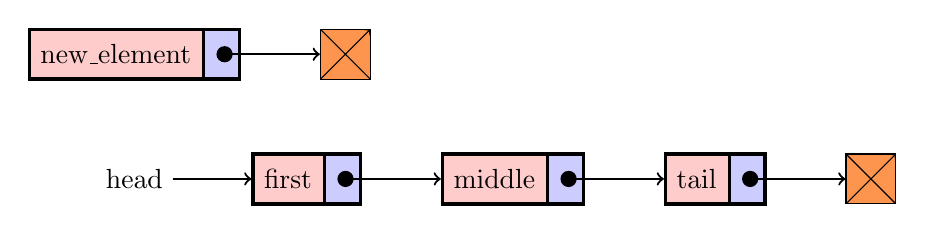
\begin{tikzpicture}
				\node (head) {head};
				\node[list,on chain] (A) [right=of head]{first};
				\node[list,on chain] (B) {middle};
				\node[list,on chain] (C) {tail};
				\node[squarecross]   (D) [right=of C] {};
				\node[list,on chain] (E) [above=of head] {new\_element};
				\node[squarecross]   (F) [right=of E] {};
				\draw[->, thick] (head) -- (A);
				\draw[chain_arrow] let \p1 = (A.two), \p2 = (A.center) in (\x1,\y2) -- (B);
				\draw[chain_arrow] let \p1 = (B.two), \p2 = (B.center) in (\x1,\y2) -- (C);
				\draw[chain_arrow] let \p1 = (C.two), \p2 = (C.center) in (\x1,\y2) -- (D);
				\draw[chain_arrow] let \p1 = (E.two), \p2 = (E.center) in (\x1,\y2) -- (F);
			\end{tikzpicture}
		\end{center}
	\end{frame}

	

	\begin{frame}
		\frametitle{Adding an Element at the Head}
		\begin{itemize}
			\item \lstinline|linked_list.add_head(new_element)|
			\item The new Node's \texttt{next} attribute will point to the old head
			\item The head will now point to the new Node
			\item Be careful with the order of operations
		\end{itemize}
		\vspace{0.7cm}
		\begin{center}
			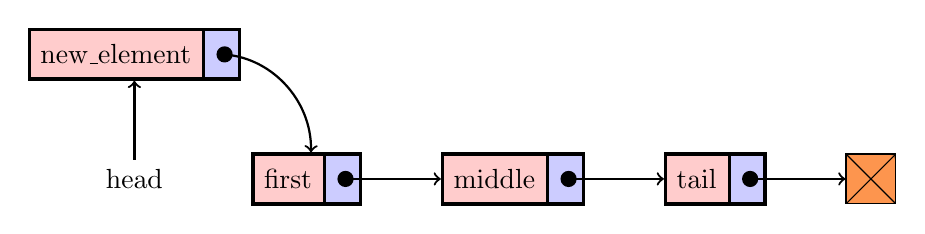
\begin{tikzpicture}
				\node (head) {head};
				\node[list,on chain] (A) [right=of head]{first};
				\node[list,on chain] (B) {middle};
				\node[list,on chain] (C) {tail};
				\node[squarecross]   (D) [right=of C] {};
				\node[list,on chain] (E) [above=of head] {new\_element};
				\draw[->, thick] (head) -- (E);
				\draw[chain_arrow] let \p1 = (A.two), \p2 = (A.center) in (\x1,\y2) -- (B);
				\draw[chain_arrow] let \p1 = (B.two), \p2 = (B.center) in (\x1,\y2) -- (C);
				\draw[chain_arrow] let \p1 = (C.two), \p2 = (C.center) in (\x1,\y2) -- (D);
				\draw[chain_arrow] let \p1 = (E.two), \p2 = (E.center) in (\x1,\y2) to [bend left=45] (A);
			\end{tikzpicture}
		\end{center}
	\end{frame}

	\begin{frame}[fragile]
		\frametitle{Adding an Element at the Head II}
\begin{lstlisting}
def add_head(self, item):
	new_node = Node(item, self.__head)
	self.__head = new_node
\end{lstlisting}
	\end{frame}

	\begin{frame}
		\frametitle{Adding an Element at the Tail}
		\begin{itemize}
			\item \lstinline|linked_list.add_tail(new_element)|
			\item Starting from the head traverse the list until we find the end
			\begin{itemize}
				\item The tail Node will have the \texttt{next} attribute set to \lstinline|None|
			\end{itemize}
			\item Modify the \texttt{next} attribute of the tail to point towards the new Node
		\end{itemize}
		\vspace{0.7cm}
		\begin{center}
			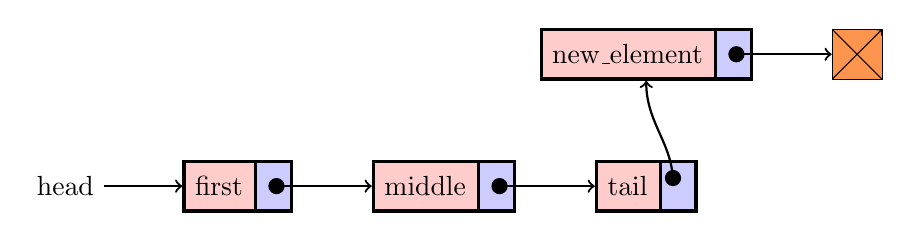
\begin{tikzpicture}
				\node (head) {head};
				\node[list,on chain] (A) [right=of head]{first};
				\node[list,on chain] (B) {middle};
				\node[list,on chain] (C) {tail};
				\node[list,on chain] (E) [above=of C] {new\_element};
				\node[squarecross]   (F) [right=of E] {};
				\draw[->, thick] (head) -- (A);
				\draw[chain_arrow] let \p1 = (A.two), \p2 = (A.center) in (\x1,\y2) -- (B);
				\draw[chain_arrow] let \p1 = (B.two), \p2 = (B.center) in (\x1,\y2) -- (C);
				\draw[chain_arrow] let \p1 = (C.two), \p2 = (C.center) in (\x1,\y2) to [out=90, in=270] (E.south);
				\draw[chain_arrow] let \p1 = (E.two), \p2 = (E.center) in (\x1,\y2) -- (F);
			\end{tikzpicture}
		\end{center}
	\end{frame}

	\begin{frame}[fragile]
		\frametitle{Adding an Element at the Tail II}
\begin{lstlisting}
def add_tail(self, item):
	if self.__head is None:
		self.__head = Node(item)
	else:
		current = self.__head
		while current.next is not None:
			current = current.next
		current.next = Node(item)
\end{lstlisting}
\end{frame}

	\begin{frame}
		\frametitle{Adding an Element after an Index}
		\begin{itemize}
			\item \lstinline|linked_list.add_after(index, new_element)|
			\item Starting from the head traverse the list and find the Node at \texttt{index} position
			\item Set the new Node's \texttt{next} attribute to the \texttt{next} of the Node at index
			\item Modify the \texttt{next} attribute of the Node at \texttt{index} to point towards the new Node
		\end{itemize}
		\vspace{0.7cm}
		\begin{center}
			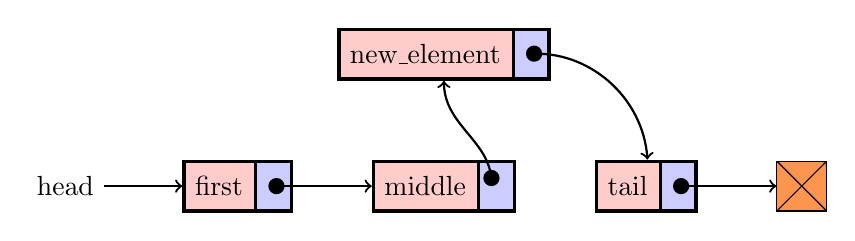
\begin{tikzpicture}
				\node (head) {head};
				\node[list,on chain] (A) [right=of head]{first};
				\node[list,on chain] (B) {middle};
				\node[list,on chain] (C) {tail};
				\node[squarecross]   (D) [right=of C] {};
				\node[list,on chain] (E) [above=of B] {new\_element};
				\draw[->, thick] (head) -- (A);
				\draw[chain_arrow] let \p1 = (A.two), \p2 = (A.center) in (\x1,\y2) -- (B);
				\draw[chain_arrow] let \p1 = (B.two), \p2 = (B.center) in (\x1,\y2) to [out=90, in=270] (E.south);
				\draw[chain_arrow] let \p1 = (C.two), \p2 = (C.center) in (\x1,\y2) -- (D);
				\draw[chain_arrow] let \p1 = (E.two), \p2 = (E.center) in (\x1,\y2) to [bend left=45] (C);
			\end{tikzpicture}
		\end{center}
	\end{frame}

	\begin{frame}[fragile]
		\frametitle{Adding an Element after an Index II}
\begin{lstlisting}
def add_after(self, index: int, item):
	current = self.__head
	for _ in range(index):
		current = current.next
	new_node = Node(item, current.next)
	current.next = new_node
\end{lstlisting}
	\end{frame}

\section{Removing Elements}

	\begin{frame}
		\frametitle{Removing an Element}
		\begin{itemize}
			\item We want to remove a Node from the list
			\begin{itemize}
				\item At the head
				\item At the tail
				\item At an index
			\end{itemize}
			\item We will have to stop referencing the Node we want to delete
			\begin{itemize}
				\item Make the node unreachable for the chain
				\item We always follow the chain starting at the head and following the arrows
			\end{itemize}
		\end{itemize}
		\vspace{0.7cm}
		\begin{center}
			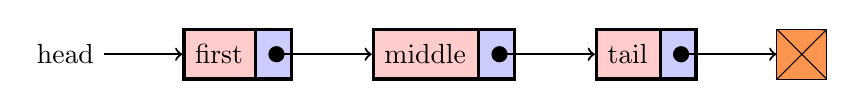
\begin{tikzpicture}
				\node (head) {head};
				\node[list,on chain] (A) [right=of head]{first};
				\node[list,on chain] (B) {middle};
				\node[list,on chain] (C) {tail};
				\node[squarecross]   (D) [right=of C] {};
				\draw[->, thick] (head) -- (A);
				\draw[chain_arrow] let \p1 = (A.two), \p2 = (A.center) in (\x1,\y2) -- (B);
				\draw[chain_arrow] let \p1 = (B.two), \p2 = (B.center) in (\x1,\y2) -- (C);
				\draw[chain_arrow] let \p1 = (C.two), \p2 = (C.center) in (\x1,\y2) -- (D);
			\end{tikzpicture}
		\end{center}
	\end{frame}

	\begin{frame}
		\frametitle{Removing the Head}
		\begin{itemize}
			\item \lstinline|linked_list.remove_head()|
			\item The \texttt{\_head} attribute of the linked list will stop pointing to the first element
			\begin{itemize}
				\item We set the new \texttt{\_head} to the value of the \texttt{next} attribute of the old one
				\item The old head will be unreachable
			\end{itemize}
		\end{itemize}
		\vspace{0.7cm}
		\begin{center}
			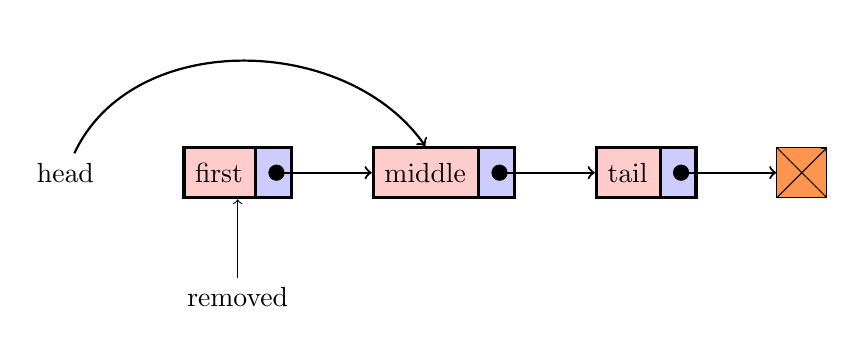
\begin{tikzpicture}
				\node (head) {head};
				\node[list,on chain] (A) [right=of head]{first};
				\node (removed) [below=of A] {removed};
				\node[list,on chain] (B) {middle};
				\node[list,on chain] (C) {tail};
				\node[squarecross]   (D) [right=of C] {};
				\draw[->, thick] (head) to [out=65, in=125] (B);
				\draw[->] (removed) -- (A);
				\draw[chain_arrow] let \p1 = (A.two), \p2 = (A.center) in (\x1,\y2) -- (B);
				\draw[chain_arrow] let \p1 = (B.two), \p2 = (B.center) in (\x1,\y2) -- (C);
				\draw[chain_arrow] let \p1 = (C.two), \p2 = (C.center) in (\x1,\y2) -- (D);
			\end{tikzpicture}
		\end{center}
	\end{frame}

	\begin{frame}[fragile]
		\frametitle{Removing the Head II}
\begin{lstlisting}
def remove_head(self):
	if self.__head is not None:
		self.__head = self.__head.next
\end{lstlisting}
	\end{frame}

	\begin{frame}
		\frametitle{Removing the Tail}
		\begin{itemize}
			\item \lstinline|linked_list.remove_tail()|
			\item We have to find the Node which \texttt{next} attribute points to the tail
			\begin{itemize}
				\item We set that Node's \texttt{next} attribute to \lstinline|None|
			\end{itemize}
		\end{itemize}
		\vspace{0.7cm}
		\begin{center}
			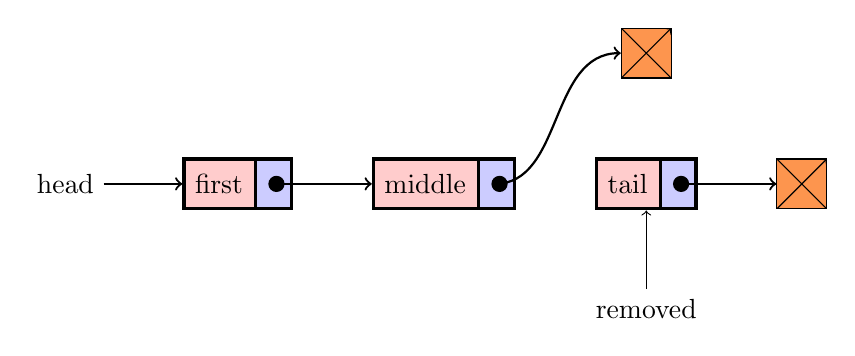
\begin{tikzpicture}
				\node (head) {head};
				\node[list,on chain] (A) [right=of head]{first};
				\node[list,on chain] (B) {middle};
				\node[list,on chain] (C) {tail};
				\node (removed) [below=of C] {removed};
				\node[squarecross]   (D) [right=of C] {};
				\node[squarecross]   (F) [above=of C] {};
				\draw[->, thick] (head) -- (A);
				\draw[->] (removed) -- (C);
				\draw[chain_arrow] let \p1 = (A.two), \p2 = (A.center) in (\x1,\y2) -- (B);
				\draw[chain_arrow] let \p1 = (B.two), \p2 = (B.center) in (\x1,\y2) to [out=0, in=180] (F);
				\draw[chain_arrow] let \p1 = (C.two), \p2 = (C.center) in (\x1,\y2) -- (D);
			\end{tikzpicture}
		\end{center}
	\end{frame}

	\begin{frame}[fragile]
		\frametitle{Removing the Tail II}
\begin{lstlisting}
def remove_tail(self):
	if self.__head is None:
		return None
	if self.__head.next is None:
		self.__head = None
	else:
		current = self.__head
		while current.next.next is not None:
			current = current.next
		current.next = None
\end{lstlisting}
	\end{frame}

	\begin{frame}
		\frametitle{Removing at an Index}
		\begin{itemize}
			\item \lstinline|linked_list.remove(index)|
			\item We have to find the Node which \texttt{next} attribute points to the Note at the index
			\begin{itemize}
				\item We set that Node's \texttt{next} attribute to the value of the \texttt{next} attribute of the Node we want to delete
			\end{itemize}
		\end{itemize}
		\vspace{0.7cm}
		\begin{center}
			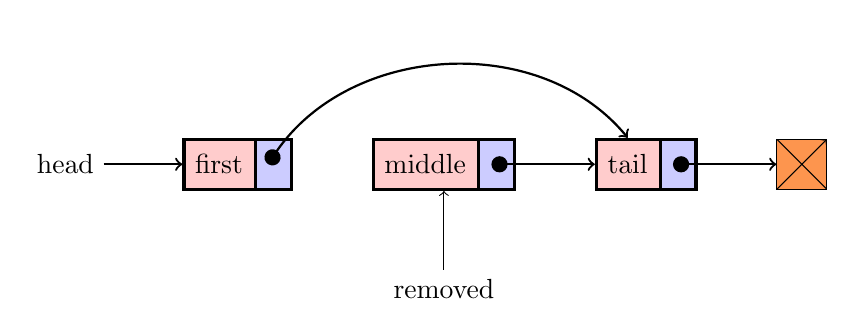
\begin{tikzpicture}
				\node (head) {head};
				\node[list,on chain] (A) [right=of head]{first};
				\node[list,on chain] (B) {middle};
				\node (removed) [below=of B] {removed};
				\node[list,on chain] (C) {tail};
				\node[squarecross]   (D) [right=of C] {};
				\draw[->, thick] (head) -- (A);
				\draw[->] (removed) -- (B);
				\draw[chain_arrow] let \p1 = (A.two), \p2 = (A.center) in (\x1,\y2) to [bend left=55] (C);
				\draw[chain_arrow] let \p1 = (B.two), \p2 = (B.center) in (\x1,\y2) -- (C);
				\draw[chain_arrow] let \p1 = (C.two), \p2 = (C.center) in (\x1,\y2) -- (D);
			\end{tikzpicture}
		\end{center}
	\end{frame}

	\begin{frame}[fragile]
		\frametitle{Removing at an Index II}
\begin{lstlisting}
def remove_index(self, index: int):
	if self.__head is None:
		return None
	if index == 0:
		self.remove_head()
	else:
		current = self.__head
		prev = None
		for i in range(index):
			prev = current
			current = current.next
		prev.next = current.next
\end{lstlisting}
	\end{frame}

	\begin{frame}
	\frametitle{Removing a Specific Element}
		\begin{itemize}
            \item We can also use a method that instead of removing an element at a given index, takes the element itself
            \item We will have to traverse the list searching for a Node with the correct data attribute
            \begin{itemize}
                \item We will have to stop with a reference to a node that is before the one we want to remove
            \end{itemize}
            \item At this point we use a process similar to removing after an index
        \end{itemize}
     \end{frame}
                
    \begin{frame}[fragile]\frametitle{Removing a Specific Element II}
\begin{lstlisting}[basicstyle=\footnotesize]
def remove(self, item):
	if self.__head is None:
		return None
	current = self.__head
	prev = None
	found = False
	while not found and current.next is not None:
		if current.data == item:
			found = True
		else:
			prev = current
			current = current.next
	if found:
		if prev is None:
			self.remove_head()
		else:
			prev.next = current.next
\end{lstlisting}
    \end{frame}

\section{Improvements}

	\begin{frame}
		\frametitle{Recommended Changes}
		\begin{itemize}
			\item If remove functions return the removed element they will work similarly to \texttt{pop()} in a \texttt{list} 
			\item Keep a counter in the class to know the number of elements, this way we do not have to traverse the list to know the size 
			\begin{itemize}
				\item Each time an item is added to the list add 1 to the counter
				\item Each time an item is removed from the list subtract 1 to the counter
			\end{itemize}
		\end{itemize}
	\end{frame}

	\begin{frame}
		\frametitle{Error Handling}
		\begin{itemize}
			\item The code we have seen does not cover error handling for some cases
			\begin{itemize}
				\item What happens if we try to call \lstinline|linked_list.add_after(100, new_element)| to a list that only has 5 elements?
				\item Should we raise an exception?
				\item Use the return statement to show if the function was successful? 
			\end{itemize}
		\end{itemize}
	\end{frame}

	\begin{frame}[fragile]
		\frametitle{Dunder methods}
		\begin{itemize}
			\item Python offers some methods to improve the functionality of a class
			\begin{itemize}
				\item They are called \href{https://docs.python.org/3/reference/datamodel.html#special-method-names}{{\color{blue}\underline{dunder or magic}}} methods, the methods are surrounded by double underscores
			\end{itemize}
			\item Show a representation of the linked list when printing like a normal \texttt{list}
			\begin{itemize}
				\item Implement the \lstinline|__str__(self)| function and return a \texttt{string}
			\end{itemize}
			\item Be able to use \lstinline|len(linked_list)| to obtain the number of elements
			\begin{itemize}
				\item Implement the \lstinline|__len__(self)| function and return the size
			\end{itemize}
			\item There are more, have a look at them and try to implement them
		\end{itemize}
	\end{frame}













\end{document}






